\chapter{Double Scenario Classification of the last shared app, KFold Validation}Starting with fitting randomly the classifiers, there are some statistics of the data used for the first test: \\
 {\def\arraystretch{1.3} 
 \begin{table}[H] 
\centering 
\begin{tabular}{|l|l|l|} 
\hline 
  &count train  &count test  \\ \hline
messenger  &302  &748  \\ \hline
telegram  &314  &736  \\ \hline
whatsapp  &340  &710  \\ \hline
original  &94  &256  \\ \hline
\end{tabular} 
\end{table} }
\section{Logistic regression results:} 
Confusion matrix with number of sample and with normalization:
 {\def\arraystretch{1.3} 
 \begin{table}[H] 
\centering 
\begin{tabular}{|l|l|l|l|l|} 
\hline 
  &messenger  &telegram  &whatsapp  &original  \\ \hline
messenger  &741  &0  &7  &0  \\ \hline
telegram  &0  &676  &60  &0  \\ \hline
whatsapp  &1  &226  &480  &3  \\ \hline
original  &0  &0  &8  &248  \\ \hline
\end{tabular} 
\end{table} }

 \begin{figure}[H] 
\centering 
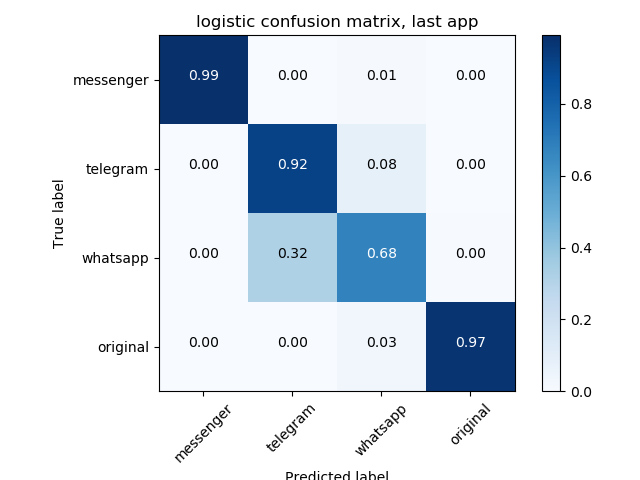
\includegraphics[scale=.6]{images/lr_initial_double_simple.png} 
\caption{logistic regression, last app classified} 
\end{figure} 


Result of the KFold validation with 10 bins:
 {\def\arraystretch{1.3} 
 \begin{table}[H] 
\centering 
\begin{tabular}{|l |l |l |l |l |l |l |l |l |l |}  
\hline 
0.9048&
0.8190&
0.9143&
0.8571&
0.8476&
0.9429&
0.8857&
0.9048&
0.8381&
0.8762\\ \hline  

\end{tabular} 
\end{table} }

The mean is : 0.879048\section{Linear Support Vector Machine results:} 
Confusion matrix with number of sample and with normalization:
 {\def\arraystretch{1.3} 
 \begin{table}[H] 
\centering 
\begin{tabular}{|l|l|l|l|l|} 
\hline 
  &messenger  &telegram  &whatsapp  &original  \\ \hline
messenger  &740  &1  &7  &0  \\ \hline
telegram  &0  &601  &135  &0  \\ \hline
whatsapp  &1  &202  &504  &3  \\ \hline
original  &0  &0  &8  &248  \\ \hline
\end{tabular} 
\end{table} }

 \begin{figure}[H] 
\centering 
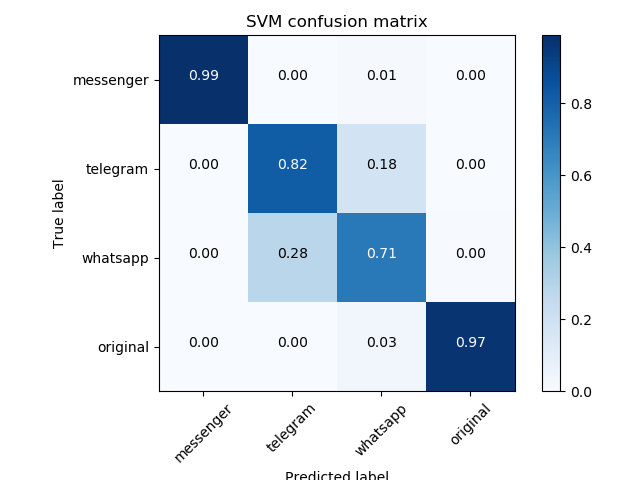
\includegraphics[scale=.6]{images/lsvm_initial_double_simple.png} 
\caption{linear SVM, last app classified} 
\end{figure} 


Result of the KFold validation with 10 bins:
 {\def\arraystretch{1.3} 
 \begin{table}[H] 
\centering 
\begin{tabular}{|l |l |l |l |l |l |l |l |l |l |}  
\hline 
0.8381&
0.7905&
0.8762&
0.8667&
0.8190&
0.8857&
0.8381&
0.8762&
0.8000&
0.8571\\ \hline  

\end{tabular} 
\end{table} }

The mean is : 0.844762\section{Random forest results:} 
Confusion matrix with number of sample and with normalization:
 {\def\arraystretch{1.3} 
 \begin{table}[H] 
\centering 
\begin{tabular}{|l|l|l|l|l|} 
\hline 
  &messenger  &telegram  &whatsapp  &original  \\ \hline
messenger  &743  &0  &5  &0  \\ \hline
telegram  &0  &589  &147  &0  \\ \hline
whatsapp  &1  &233  &473  &3  \\ \hline
original  &1  &0  &2  &253  \\ \hline
\end{tabular} 
\end{table} }

 \begin{figure}[H] 
\centering 
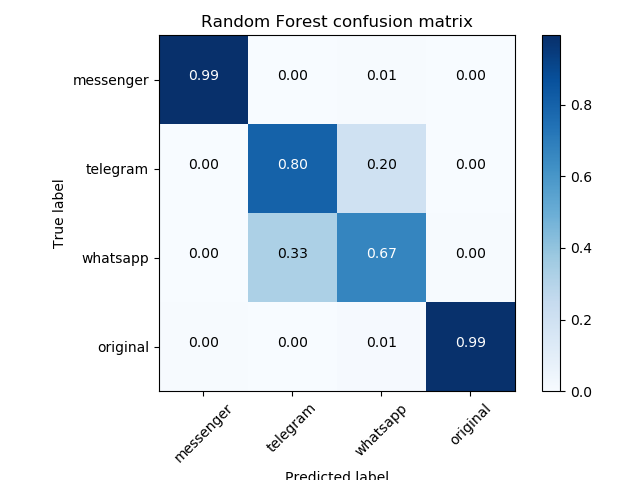
\includegraphics[scale=.6]{images/rf_initial_double_simple.png} 
\caption{random forest, last app classified} 
\end{figure} 


Result of the KFold validation with 10 bins:
 {\def\arraystretch{1.3} 
 \begin{table}[H] 
\centering 
\begin{tabular}{|l |l |l |l |l |l |l |l |l |l |}  
\hline 
0.8286&
0.8190&
0.8762&
0.8952&
0.8381&
0.8762&
0.8286&
0.8476&
0.8571&
0.8381\\ \hline  

\end{tabular} 
\end{table} }

The mean is : 0.850476